%!TEX encoding = UTF-8 Unicode

\documentclass[code,math,bibliography]{relatorio-deti}
\usepackage{xurl}

\title{GSMA Open Gateway\\[20pt]Technical Report}
\cadeira{Software Engineering Final Project}
\relatorioAno{2025}

\membro{Luís Godinho}{112959}
\membro{Igor Coelho}{113532}
\membro{João Capucho}{113713}
\membro{Zakhar Kruptsala}{114478}
\membro{Filipe Sousa}{114196}

\addbibresource{bibliography.bib}

\usepackage{lmodern}

\begin{document}

\maketitle

% TODO
%\chapter*{\Large\centering Agradecimentos}
%\thispagestyle{empty}
%
%Gostaríamos de expressar os nossos agradecimentos aos nossos orientadores, o
%Professor Rafael Direito e o Professor Diogo Gomes por nos terem guiado na
%realização deste projeto ao longo do semestre, garantindo o seu sucesso.
%
%\clearpage

\chapter*{\Large\centering Resumo}
\thispagestyle{empty}

O GSMA Open Gateway é uma iniciativa a escala global que pretende oferecer a
desenvolvedores acesso às redes 5G dos operadores de telecomunicações. Este
acesso permite desenvolver soluções que conseguiriam aceder a informações da
rede e reconfigurá-la de modo a oferecer aos utilizadores finais experiências
integradas. Estas consistem em utilizar a integração com a rede para melhorar
casos de uso existentes e suportar novos casos de uso, como a deteção de
fraude, \emph{Quality-on-Demand} e gestão avançada de frota. O acesso é feito
via um conjunto de interfaces programáticas que unificam e simplificam as
interfaces existentes dos operadores, tendo em conta também a legislação
existente em questões de privacidade e proteção de dados.

Apesar da maioria dos operadores não oferecer estas interfaces, é expectável
que as venham oferecer no futuro, havendo assim a necessidade dos
desenvolvedores começarem a projetar integrações com estas. O nosso projeto
consiste em oferecer uma implementação destas interfaces através da
infraestrutura 5G do \emph{Instituto de Telecomunicações} em Aveiro.

\vspace{1cm}

\noindent\textbf{Palavras-chave:} Redes 5G, Infraestruturas Cloud


\tableofcontents

\clearpage

\chapter{Introduction}

\section{Context}

The development of 5G networks and beyond 5G have introduced
advanced capabilities in the access, reconfiguration and
flexibility of these networks. This attracts the interest of
software developers in several industries, aiming to offer
integrated solutions to their clients that leverage these
capabilities of the network and their operators. However, the
existing interfaces currently defined by the \emph{3rd Generation
Partnership Project} (\emph{3GPP}) expose much of the complexity
related to the networks and the operators. This complexity
hinders the development of integrated solutions and requires
extensive knowledge on the topic of networks and how to operate
them, limiting the adoption.

The \emph{GSMA Open Gateway} is an industry initiative to solve
this problem. This is done by a set of Application Programming
Interfaces (API) defined by the \emph{CAMARA} project, that
exposes various simplified interfaces of the operator networks.
These APIs can then be offered either through the MNOs directly
or by aggregators, such as \emph{Hyperscalers}.

However, most operatiors do not offer said interfaces, but it is
to be expected that they will do so in the near future. Given the
capabilities of \emph{Instituto de Telecomunicações} (IT) in
Aveiro, with access to a 5G infrastructure
\footnote{\url{https://5gainer.eu/}}\cite{ieee:5GAIner}, there is 
interest in integrating \emph{GSMA Open Gateway} APIs in their
offer.

\section{Goals}

The objectives outlined for the project were as follows:

\begin{enumerate} 
  \item Implemetation of the following \emph{GSMA
      Open Gateway} \emph{APIs} through integration with
      \emph{IT's} 5G Core. 
    \begin{itemize}
      \item \emph{API} family to obtain \emph{Device Information}
      \item \emph{API} family to obtain information on the
        network's \emph{Quality-of-Service} (\emph{QoS}) and to
        offer \emph{QoS-on-Demand} (\emph{QoD}).
    \end{itemize}

  \item Implementation of the \emph{GSMA
    Open Gateway} \emph{API} to obtain and verify \emph{One Time
    Passwords} (\emph{OTP}) through \emph{SMS}, utilizing an 
    \emph{SMS Centre} (\emph{SMSC}) integrated in \emph{IT's} 5G
    Network as a part of our project.

  \item Implementation of the \emph{GSMA Open Gateway APIs} to
    offer location through the \emph{NEFSim} project, an emulator
    of the \emph{Network Exposure Function} (\emph{NEF},
    explained in more detail in section
    \ref{sec:related_work_3gpp}) The utilization of this emulator
    is required, since \emph{IT's} network currently does not have
    such a service in its infrastructure.

  \item Integration of our project with the 
    \emph{OpenSlice}\footnote{\url{https://osl.etsi.org/}}, an
    \emph{Operation Support System} (\emph{OSS}), allowing for
    the usage of a \emph{CAMARA as a Service} (\emph{CAMARAaaS})
    business model.

  % \item Integration of the \emph{Common API Framework}
  %   (\emph{CAPIF}) with our project, through \emph{OpenCAPIF}, to
  %   control the exposure and consumption of our \emph{APIs}

\end{enumerate}


\chapter{State of the Art}

\section{Related Work}

This section aims to present projects in the same field of work,
or at least with similar objectives to our own, the relationship
between these other projects and ours, and how they compare.

\subsection{3GPP OpenAPIs}\label{sec:related_work_3gpp}

\emph{3GPP}, the body responsible for the norms that define the
5G protocol, designed not only the radio interface to be used by
5G Networks (designated \emph{5G New Radio}, shortened as
\emph{5G-NR}), but also the architecture of the network's
\emph{Core}. This new architecture is a \emph{Service-Based
Architecture}, with each service denominated as \emph{Network
Functions} (\emph{NFs}). These consist of applications that run
on generic hardware, such as the one offered by Cloud
Infrastructure.

These services communicate between them by \emph{APIs} defined by
\emph{3GPP} and described in \emph{OpenAPIs}, a documentation
standard. However, these \emph{APIs} are designed for use only
inside the MNO's network \emph{core}, and not to be used by third
parties, exception being made to the \emph{Network Exposure
Function} (\emph{NEF}). The latter, is an \emph{NF} specifically
designed to allow third-party access to the MNO's network
capabilities securely. The \emph{APIs} that are offered are
designated as \emph{Northbound Interfaces}, and their clients are
denominated of \emph{Application Functions} (\emph{AFs}).

In conclusion, 3GPP OpenAPIs operate only in the operator's
domain and do not expose the operator's network capabilities to
third parties, exception being made to the \emph{NEF}, whose
purpose is to explicitly support network integration by
third-parties with MNO's. Even if a MNO decides to directly
expose the \emph{3GPP} designed APIs, software developers would
not be capable of using them, since these are limited to the
scope of the network, therefore using them requires extensive
domain-specific knowledge.

\subsection{CAMARA}

The \emph{CAMARA} initiative's main objectives are the
definition, development and validation of
\emph{Network-as-a-Service} (\emph{NaaS}) \emph{APIs}. These are
being developed with focus on rapid implementation, in order to
achieve one of \emph{CAMARA}'s big objectives, which is MNO
adoption, as a way to ensure an unified interface that is not
supplier dependent and that is able to give third-parties the
opportunity to interact with 5G services without the need to
contact the MNO.

Another of \emph{CAMARA}'s big objectives is the accessibility of
all its APIs to software developers without any experience in the
5G/Telecom domain, that is, to ensure that the developers are
able to utilize these services simply and without the need to
interact directly with network operators or learn the details of
telecommunications to be able to use these \emph{APIs} 

This initiative is heavily related with \emph{GSMA Open Gateway},
which we will talk about in the next section, since it is these
\emph{APIs} that will be published through \emph{CAMARA}. In
addition, the GSMA Open Gateway, CAMARA and TMF are aligned to
bring 5G capabilities to the market in a more accessible and
standardized way.


\subsection{GSMA Open Gateway}

Similarly to the \emph{NEF}, the \emph{GSMA Open Gateway} aims to
expose the various capabilities of network operators to third
parties. However, there are advantages to using the \emph{GSMA
Open Gateway}:

\begin{itemize} \item \textbf{Simplification}, the NEF exposes
      quite complex interfaces with various details of the
      operator's  of the operator's network, requiring knowledge
      of mobile networks and 5G, increasing the cost of adopting
      these APIs.

    \item \textbf{Aggregation}, the NEF only exposes access to
      the operator's network, while the GSMA Open Gateway
      provides for the existence of aggregators that offer the
      APIs to various operators in an unified manner, requiring
      contact with only one aggregator rather than multiple
      operators.

\item \textbf{Privacy management}, the GSMA Open Gateway includes
mechanisms for the end-user consent, which in many cases is
necessary for legal reasons.\end{itemize}

This does not imply that \emph{NEF} is an inferior interface; it
offers greater integration with operators' networks. In reality,
\emph{NEF} and \emph{GSMA Open Gateway} are complementary
technologies. Still, it's important to note that \emph{GSMA Open
Gateway} is a more convenient interface for most third-party
application developers because, unlike direct interaction with
\emph{NEF},  it does not require knowledge of mobile networks.
The \emph{NEF} is also important, on the one hand because it
offers greater integration with the operator's network, but also
because it is possible to implement a \emph{GSMA Open Gateway}
over it, modelling it as an \emph{AF}.

\subsection{TMF Open Digital Architecture}

The \emph{Open Digital Architecture} (\emph{ODA}) is a framework
created by the \emph{TM Forum} (\emph{TMF}) to help service
providers transition to open and interoperable solutions. This
framework spans several areas, touching not only on the technical
side but also on the company's processes. In our project, the
most relevant are the \emph{OpenAPIs} defined in this framework,
which define domain-independent interfaces for offering resources
and services. Of particular interest are the interfaces that make
it possible to obtain a service catalog, acquire these services
and control their life cycle.

The \emph{TMF APIs} are more generic than those offered by the
\emph{GSMA Open Gateway}, offering more operations, but also
increasing the complexity of their use compared to those offered
by the \emph{GSMA Open Gateway}. The \emph{GSMA Open Gateway}
also has the advantage of accommodating the multiple gateway
aggregation scenario, allowing an aggregator to offer access to
\emph{GSMA Open Gateway APIs} from several operators in an unified
way, without the customer having to maintain contact with each
operator individually. An interesting case in the collaboration
of these two projects is the use of \emph{TMF APIs} to allow
operators and aggregators to offer \emph{GSMA Open Gateway} as a
service. In this scenario, the \emph{TMF APIs} would be used to
offer the customer the opportunity to purchase a service that
would provide a \emph{GSMA Open Gateway}. This would be
orchestrated and made available in an automated way, reinforcing
the operator/aggregator's offer and simplifying the developer's
process of gaining access to the \emph{GSMA Open Gateway}.


\section{\emph{API} Adoption} Although these initiatives are
relatively new, there are already operators implementing the
\emph{APIs} defined by \emph{CAMARA} and the \emph{GSMA Open
Gateway}.

\emph{Ericsson}, a multinational telecommunications company, has
started to implement the \emph{APIs} defined by the \emph{CAMARA}\footnote{\url{https://www.fierce-network.com/wireless/ericsson-leads-top-operators-new-global-api-venture}} project, along with companies such as \emph{Google Cloud},
\emph{Deutsche Telekom}, \emph{Reliance Jio} and
\emph{T-Mobile}\footnote{\url{https://adunaglobal.com/\#mission}},
participating in an initiative called \emph{Aduna}, which is
developing and adopting a set of CAMARA APIs. The first APIs to
be supported will be focused mainly on fraud prevention, with the
aim of verifying numbers assigned to customers and an API that
aims to facilitate the SIM Swapping
process\footnote{\url{https://www.fierce-network.com/wireless/what-will-aduna-ericssons-massive-api-venture-release-first}}.

Similarly, in the Middle East and North Africa region, an
operator, \emph{Ooredoo}, recently implemented \emph{CAMARA
APIs}, allowing the offer of new opportunities to businesses
(customers)\footnote{\url{https://www.ooredoo.com/en/media/news_view/ooredoo-group-leads-mena-with-gsma-camara-api-implementation/}}.

This reaffirms the commitment that the various operators have
made to the \emph{GSMA Open Gateway} and the \emph{CAMARA}
initiative.

Like \emph{Aduna}, \emph{Ooredoo} has also started to offer
programmatic \emph{SIM Swapping}, as well as providing the
necessary support for implementing One Time Password (OTP) via
SMS. Finally, the four main mobile operators in France
(\emph{Bouygues Telecom}, \emph{Free}, \emph{Orange} and
\emph{SFR}) announced a partnership to launch network \emph{APIs}
to help fight online fraud and protect digital identities. As
part of the \emph{GSMA Open Gateway} global initiative, they will
make three APIs available on the French market, namely \emph{Know
Your Customer (KYC) Match}, \emph{SIM Swapping} and \emph{Number
Verification}. These have been tested with banks and companies in
France and should be launched commercially in the first half of
2025\footnote{\url{https://www.gsma.com/newsroom/press-release/french-mobile-industry-accelerates-deployment-of-network-apis-through-gsma-open-gateway-initiative/}}.


\chapter{System Requirements}

When any system is developed, it aims to make different use cases possible,
which are carried out by one or more actors. These actors, who interact
directly with the system, have requirements that need fulfilling, i.e.,
functionalities that the system must have in order to meet their needs. As
such, it is necessary to survey these requirements in order to better develop
the system to meet the needs of its users.

Thus, in this chapter we will not only present the actors who will interact
with the system, but also the various uses that these users will give the
system, as well as the various requirements it must meet.

\section{Actors}

As already mentioned, the creation of \emph{APIs GSMA Open Gateway} aims to
facilitate the programmatic use of the various resources and features that the
\emph{5G} network can offer. As such, the system has 2 distinct actors.
\begin{itemize}
  \item \textbf{Network operator} - The first actor to interact with the system
    is the network operator, who provides the APIs to various other businesses,
    so that they can interact with the network programmatically. However, since
    the APIs designed by the \emph{GSMA Open Gateway} are considerably simpler
    than those defined by the \emph{3GPP}, a network operator can also use
    these APIs to manage the network itself.

\item \textbf{\emph{Vertical
  Clients}}\footnote{\url{https://5g-ppp.eu/verticals/}} - The second actor to
    interact with the system is actually its target audience. Several
    businesses develop a set of products that interact with the network. These
    businesses use the APIs defined by the \emph{GSMA Open Gateway} to not only
    offer a wider range of functionalities to their users, but also to carry
    out a series of checks in order to guarantee the correct use and
    performance of their products.
\end{itemize}

\section{Use Cases}

The two actors presented in the previous section have several use cases. These
are shown in the following diagram.

\begin{figure}[H]
  \centerline{
    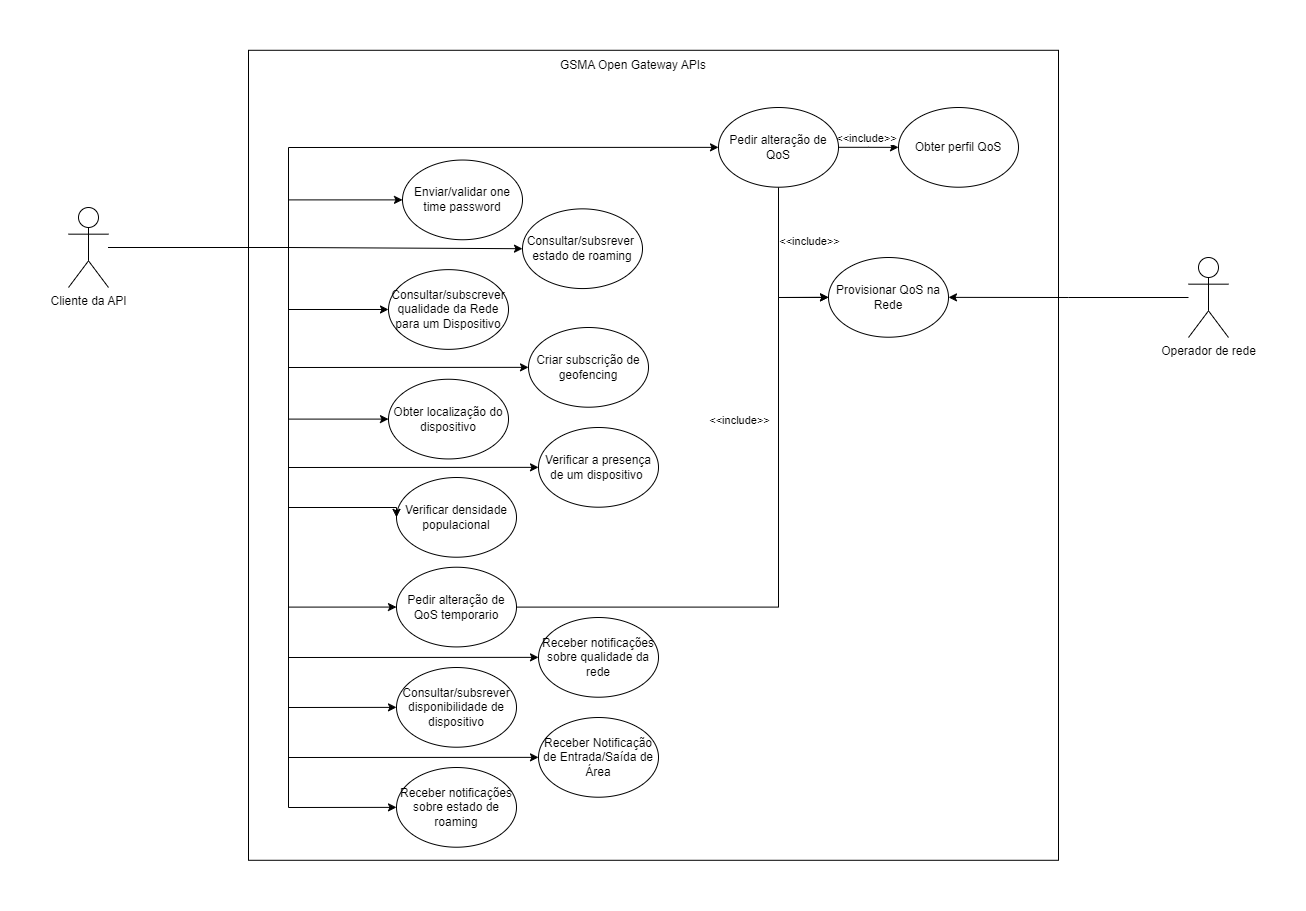
\includegraphics[width=20cm]{figs/use_case_diagram.png}
  }
  \caption{Use Case Diagram}
\end{figure}

\begin{itemize}
  \item \textbf{Network Operator}

    Although the network operator can interact directly with the \emph{5G
    core}, the network operator can use the APIs it makes available to more
    easily manage the quality of service of its network

  \item{\textbf{Vertical Clients}}

    The customers of the APIs are the various businesses that want to
    programmatically modify the network, either to offer better
    products/services to their customers, or to manipulate an internal network
    to better suit their needs. Using the APIs defined by the \emph{GSMA Open
    Gateway}, the various businesses can:
    \begin{enumerate}
      \item Send/Validate One Time Passwords (OTPs), to (for example) check the
        validity of a phone number via SMS

      \item Check or subscribe to roaming status, so you can verify whether 
        a device is in another country.

      \item Check and/or subscribe to the network quality for a given device,
        so that you know if the network requirements for the application can be
        met; if you subscribe, a notification will be sent whenever there is a
        change in quality.

      \item Obtain the location of a given device

      \item Check the presence of a device, i.e. check whether a particular
        device is within the defined area.

      \item Check the population density in a given area

      \item Request a QoS change, temporary or not, due to the need for more
        bandwidth.

      \item Receive notifications about network status

      \item Receive notifications regarding the entry or exit of a device from
        a given area

      \item Subscribe/Consult the availability of a device
    \end{enumerate}
\end{itemize}

\section{Requirements}

For the development of the system, the following requirements were gathered:

\subsection{Functional Requirements}

\begin{itemize}
  \item \textbf{Location Services:}
    \begin{itemize}

      \item The system must allow the creation of event subscriptions so that
        \emph{CAMARA API} clients receive notifications when they enter or leave a
        defined area.

      \item The system must make it possible to obtain the location of a
        device, this being described by a circle (coordinates of the center and
        radius) or a simple polygon (list of coordinates)

      \item The system must make it possible to check whether a device is in a
        certain area. If this area is outside the area covered by the operator
        or if this area is valid, among other things, it should return the
        correct errors.

      \item The system must make it possible to obtain an estimate of the
        population density in a specified area
    \end{itemize}

  \item \textbf{Communication Quality:}
    \begin{itemize}
      \item The system should allow the exchange of relevant information to help make
        decisions related to the network APIs.

      \item The system should allow developers to consult the network about the
        likelihood of meeting connectivity requirements in a session. 

      \item The system should allow developers to define different QoS on client APs,
        depending on their bandwidth needs.

      \item The system should allow the existing QoS profiles in a network to be
        obtained and the information relating to them to be returned.

      \item The system must allow QoS profiles to be assigned to a device. The
        network will apply the QoS profile to the device's traffic whenever it is
        connected, until this provisioning is removed.
    \end{itemize}

  \item \textbf{Fraud Protection:}
    \begin{itemize}
      \item The system must allow for the verification of a given phone number,
        through the emission and validation of an OTP.
    \end{itemize}

  \item \textbf{Device Information Gathering:}
    \begin{itemize}
      \item The system must make it possible to check whether a particular
        device is available on the network.

      \item The system must allow an API subscriber to be notified if there is
        a change in the availability of a particular device.

      \item The system must be able to check whether a particular device is
        roaming, and if so, return the existing information about the country.

      \item The system must allow an API subscriber to be notified if there is
        a change in the roaming status of a device.
    \end{itemize}
\end{itemize}

\subsection{Non-Functional Requirements}

\begin{itemize}
  \item \textbf{Performance and Latency:}
    \begin{itemize}
      \item The system should maintain consistent response times as the user base or data volume increases 

      \item The system must be able to handle an increasing number of requests.
    \end{itemize}

  \item \textbf{Scalability:}
    \begin{itemize}
      \item The system must ensure that the system supports a high volume of requests and connected devices

      \item The system must scale horizontally and/or vertically depending on demand.
    \end{itemize}

  \item \textbf{Availability and Reliability:}
    \begin{itemize} 
      \item The system must establish availability levels (e.g. 99.9\% SLA
        uptime) 

      \item The system must have a high level of reliability (i.e. 99.9999\%
        reliability)

      \item The system must have a redundancy and fault tolerance mechanism,
        guaranteeing continuous operation even under adverse conditions.
    \end{itemize}

  \item  \textbf{Interoperability:}
    \begin{itemize}
      \item The system must be compatible with different operators,
        guaranteeing the integration of APIs with the infrastructure of
        different network operators, promoting the universality of services.

      \item The system must ensure that APIs follow open standards and best
        practices, promoting interoperability and universal acceptance between
        different systems and technologies.
    \end{itemize}


  \item \textbf{Maintainability and Extensibility:}
    \begin{itemize}
      \item The system must have a modular architecture, allowing the system to
        be divided into independent components, facilitating updates and
        corrections without affecting the overall functioning.

      \item The system must have detailed documentation, with manuals, to help
        developers understand and maintain the system effectively.

      \item The system must have clean and readable code, following standards
        that make the code easy to understand and modify, reducing the
        likelihood of errors.

      \item The system should have flexibility for updates, making it easy to
        implement new features or improvements without having to rewrite large
        parts of the code.
    \end{itemize}

  \item \textbf{Usability:}
    \begin{itemize}
      \item The system should return errors, if any, following the defined
        standard, facilitating the integration of these APIs as well.

      \item The system should only return relevant information to the
        developer, abstracting them from more complex network information.
    \end{itemize}
\end{itemize}


\chapter{System Architecture}

\chapter{Gateway Development}


\section{Location Service APIs}

For the gateway we developed a set of Location APIs that we considered to be
most relevant and that were achievable with the available tools. These
consisted of the Location Retrieval, Location Verification and lastly
Geafencing Subscriptions APIs.

\subsection{Location Retrieval}

This API has a the goal of getting the location of a device with a simple API.
This location is as seen by network operators and will have varying degrees of
certainty.

The implementation uses 3GPP's Monitoring Event API with the monitoring type
set to \Verb{LOCATION_REPORTING}  with a single report. This means that instead of
sending a notification on the next location update the report is sent imediatly
on the response from where we extract the most recent information device
location information.

\subsection{Location Verification}

The Location Verification API, although it might seem similar to the previous
one has a different purpose. This API tells the caller wether a device is
within a certain area or not. This means that exact position of the device is
not relevant but only if it is or is not within a specified region.

Once again this API uses the Monitoring Event API on the NEF side to obtain the
location of the device. Having done this the gateway then calculates wether the
device is within or outside the specified region.

\subsection{Geofencing Subscription}

Finally in the Location Service collection of APIs we have the Geofencing
Subscriptions. This one is responsible for sending notifications to a given
sink. The notification is triggered everytime a device enters a given region or
whenever the device exits it depending on the configuration of the
subscription. Additionally, there are endpoints for managing the subscriptions,
allowing listing, getting details and deleting existing subscriptions.

As with the previous two APIs, this one also uses the Monitoring Event API
provided by the NEF to obtain the device location, but unlike the other ones it
actually creates a subscriptions. Internally the gateway has webhook listening
for location updates. Upon the creation of the subscription the details are
stored in a Redis instance for fast retrieval, each subscription will have a
unique identifier and, as such, when the Monitoring Event subsctipription is
created the webhook for the notification comes with that identifier. This way
when the gateway receives a notification from NEF it can distinguish between
the different subscriptions.

Once the notification is received on the gateway the location reported is
evaluated to know whether the device is or isn't inside the region and
depending on the previous known state and the configuration of the subscription
an according notification will be sent (if the conditions are met).

Along side the notification sending there are two more aspects that need
tracking which is the expire date of the subscription and the max number of
notifications. Every time a notification is sent, if a max number of
notifications is set, then a counter is incremented to stop notifications when
the limit is reached. As for the expire time, there is a seperate thread that
checks periodicly if the subscription has expired or not to flag it
accordingly.


\section{Communication Quality APIs}

We have exposed only a fundamental subset of the Communication Quality APIs on our gateway, similar to what we have done with our other sets of APIs. We chose this course of action for two reasons: one, due to the available tools IT provided us, and two, focusing on the most important capabilities for our primary use case.

Correspondingly, our implementation targets a subset of this API family: Quality on Demand, Quality on Demand Provisioning, and Quality of Service Profiles. These three services together provide dynamic quality adaptation, the provisioning of quality levels on an as-needed basis, and the specification of service profiles that ensure performance bounds for communications. By focusing our efforts there, we’ve created a lightweight, yet extremely efficient, collection of quality-management APIs that play well with our underlying infrastructure.

\subsection{Quality on Demand}

The Quality on Demand (QoD) API offers a programmable interface that allows developers to request stable latency or prioritized throughput managed directly by the network. By abstracting the complexity of underlying network technologies, the API enables developers to concentrate on optimizing user experiences for applications requiring high-performance network communication.

The solution employs 3GPP’s \emph{Nnef\_AFsessionWithQoS} interface to drive dynamic, on-demand subscription for application-level data flows. As an application client requires guaranteed QoS to a particular server, the client-side gateway collects the proper identifiers (i.e., client IP address, server IP address, port numbers) and translates them into standardized 3GPP flow description. This flow description is passed as a subscription request to the NEF (Network Exposure Function) through its \emph{Nnef\_AFsessionWithQoS} operation. The NEF checks the request against the existing network policy and available resources, and sends an authorization response stating whether the QoS resources were reserved successfully or not. If granted, the network dynamically applies the agreed QoS parameters end-to-end between the server and the application client.

In addition to session creation, the CAMARA QoD API provides functionality to manage active sessions. It allows retrieving session information by session ID or by device identifier, making it easier to monitor ongoing QoS allocations. Furthermore, the API supports extending the lifetime of existing sessions if continued QoS is required, as well as deleting sessions when QoS is no longer needed or the application session terminates.

\begin{figure}[H]
	\centerline{
		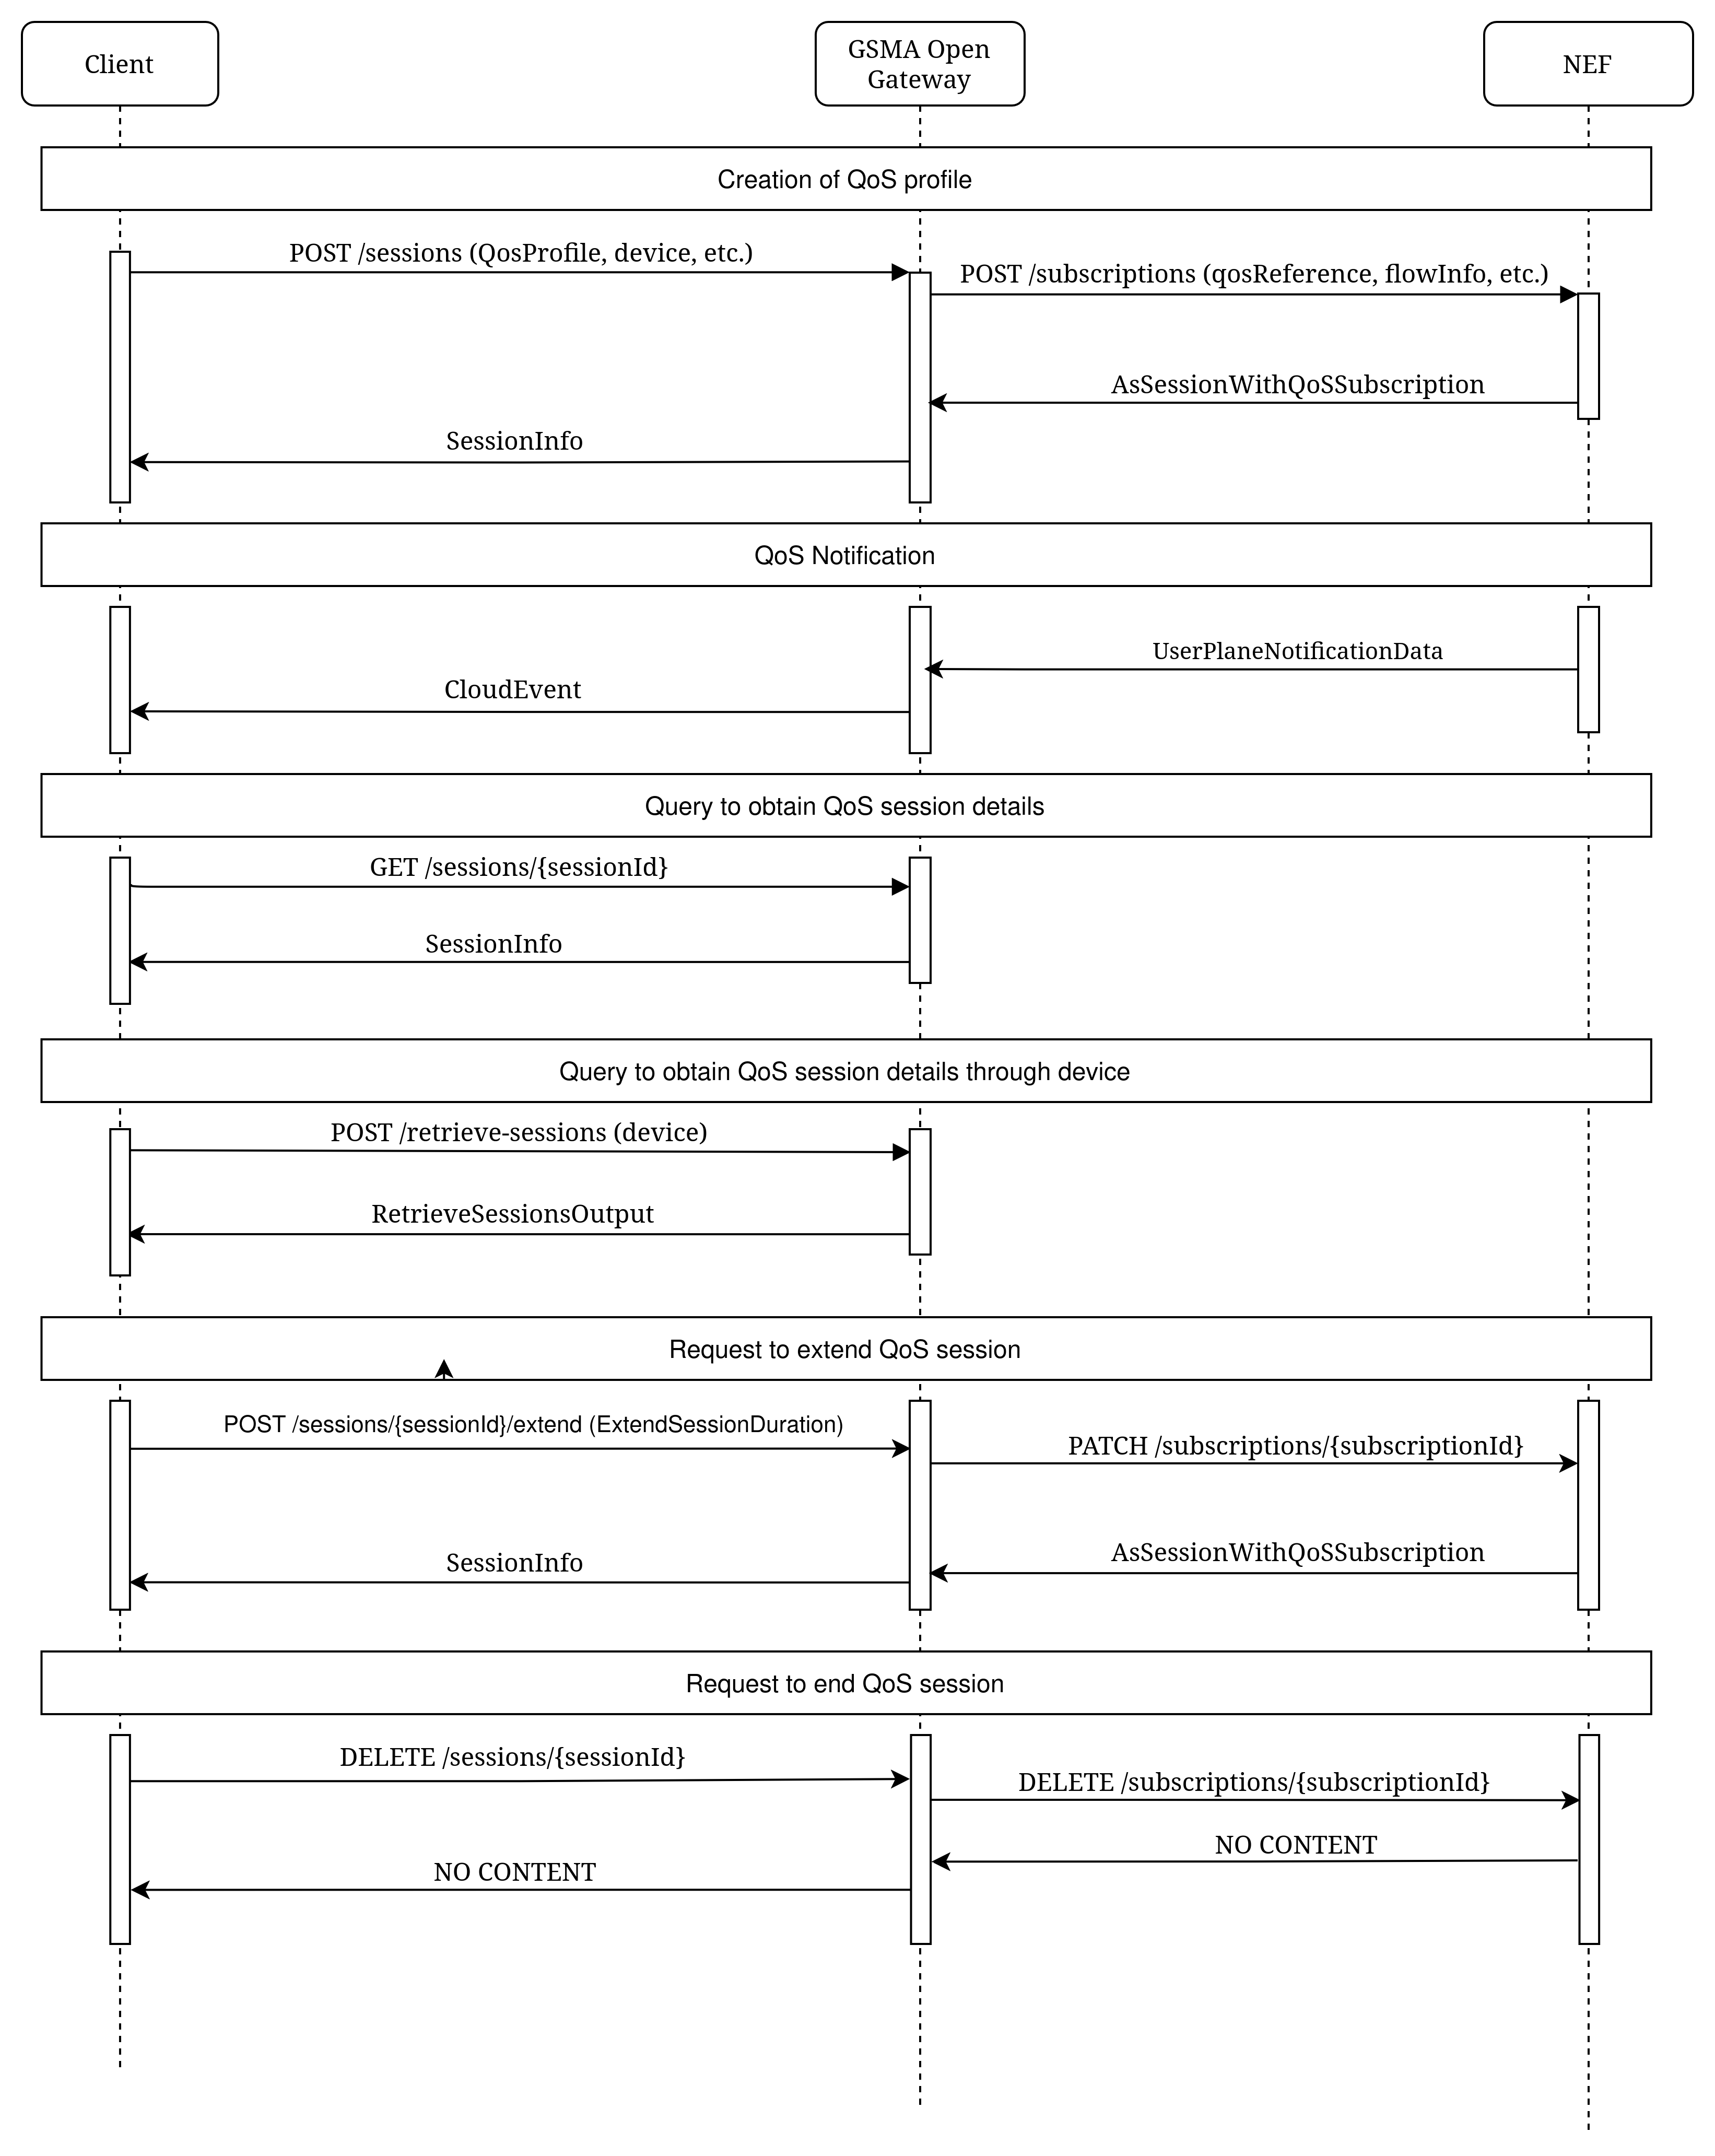
\includegraphics[width=10cm]{figs/QoD_sequence_diagram.png}
	}
	\caption{Quality on Demand Sequence Diagram}
\end{figure}

\subsection{Quality on Demand Provisioning}

The Quality On Demand Provisioning API provides a programmable interface that enables developers to assign specific Quality of Service (QoS) profiles to individual devices on a permanent basis. Once provisioned, the network applies the designated QoS profile to the device whenever it connects, maintaining the configuration until the provisioning is explicitly removed.

Similar to the previous Quality-on-Demand API, the QoD Provisioning API also leverages 3GPP’s \emph{Nnef\_AFsessionWithQoS} interface to manage QoS sessions. However, unlike the standard QoD API which typically focuses on application-level flows between clients and servers, the QoD Provisioning API is designed to allocate QoS resources directly for a specific device.

In this case, the gateway or application provides the device identity (e.g., SUPI, GPSI, or IP address) along with the requested QoS reference. The API translates this information into a 3GPP compliant request and submits it via the \emph{Nnef\_AFsessionWithQoS} interface to the NEF. The NEF evaluates network resource availability and policy constraints, and returns a response indicating whether the requested QoS resources have been successfully allocated for the device.

Similar to the QoD API, the QoD Provisioning API also provides management capabilities: it allows retrieving existing provisioning information by provisioning ID or device or deleting provisioning when the dedicated QoS is no longer required.


\begin{figure}[H]
	\centerline{
		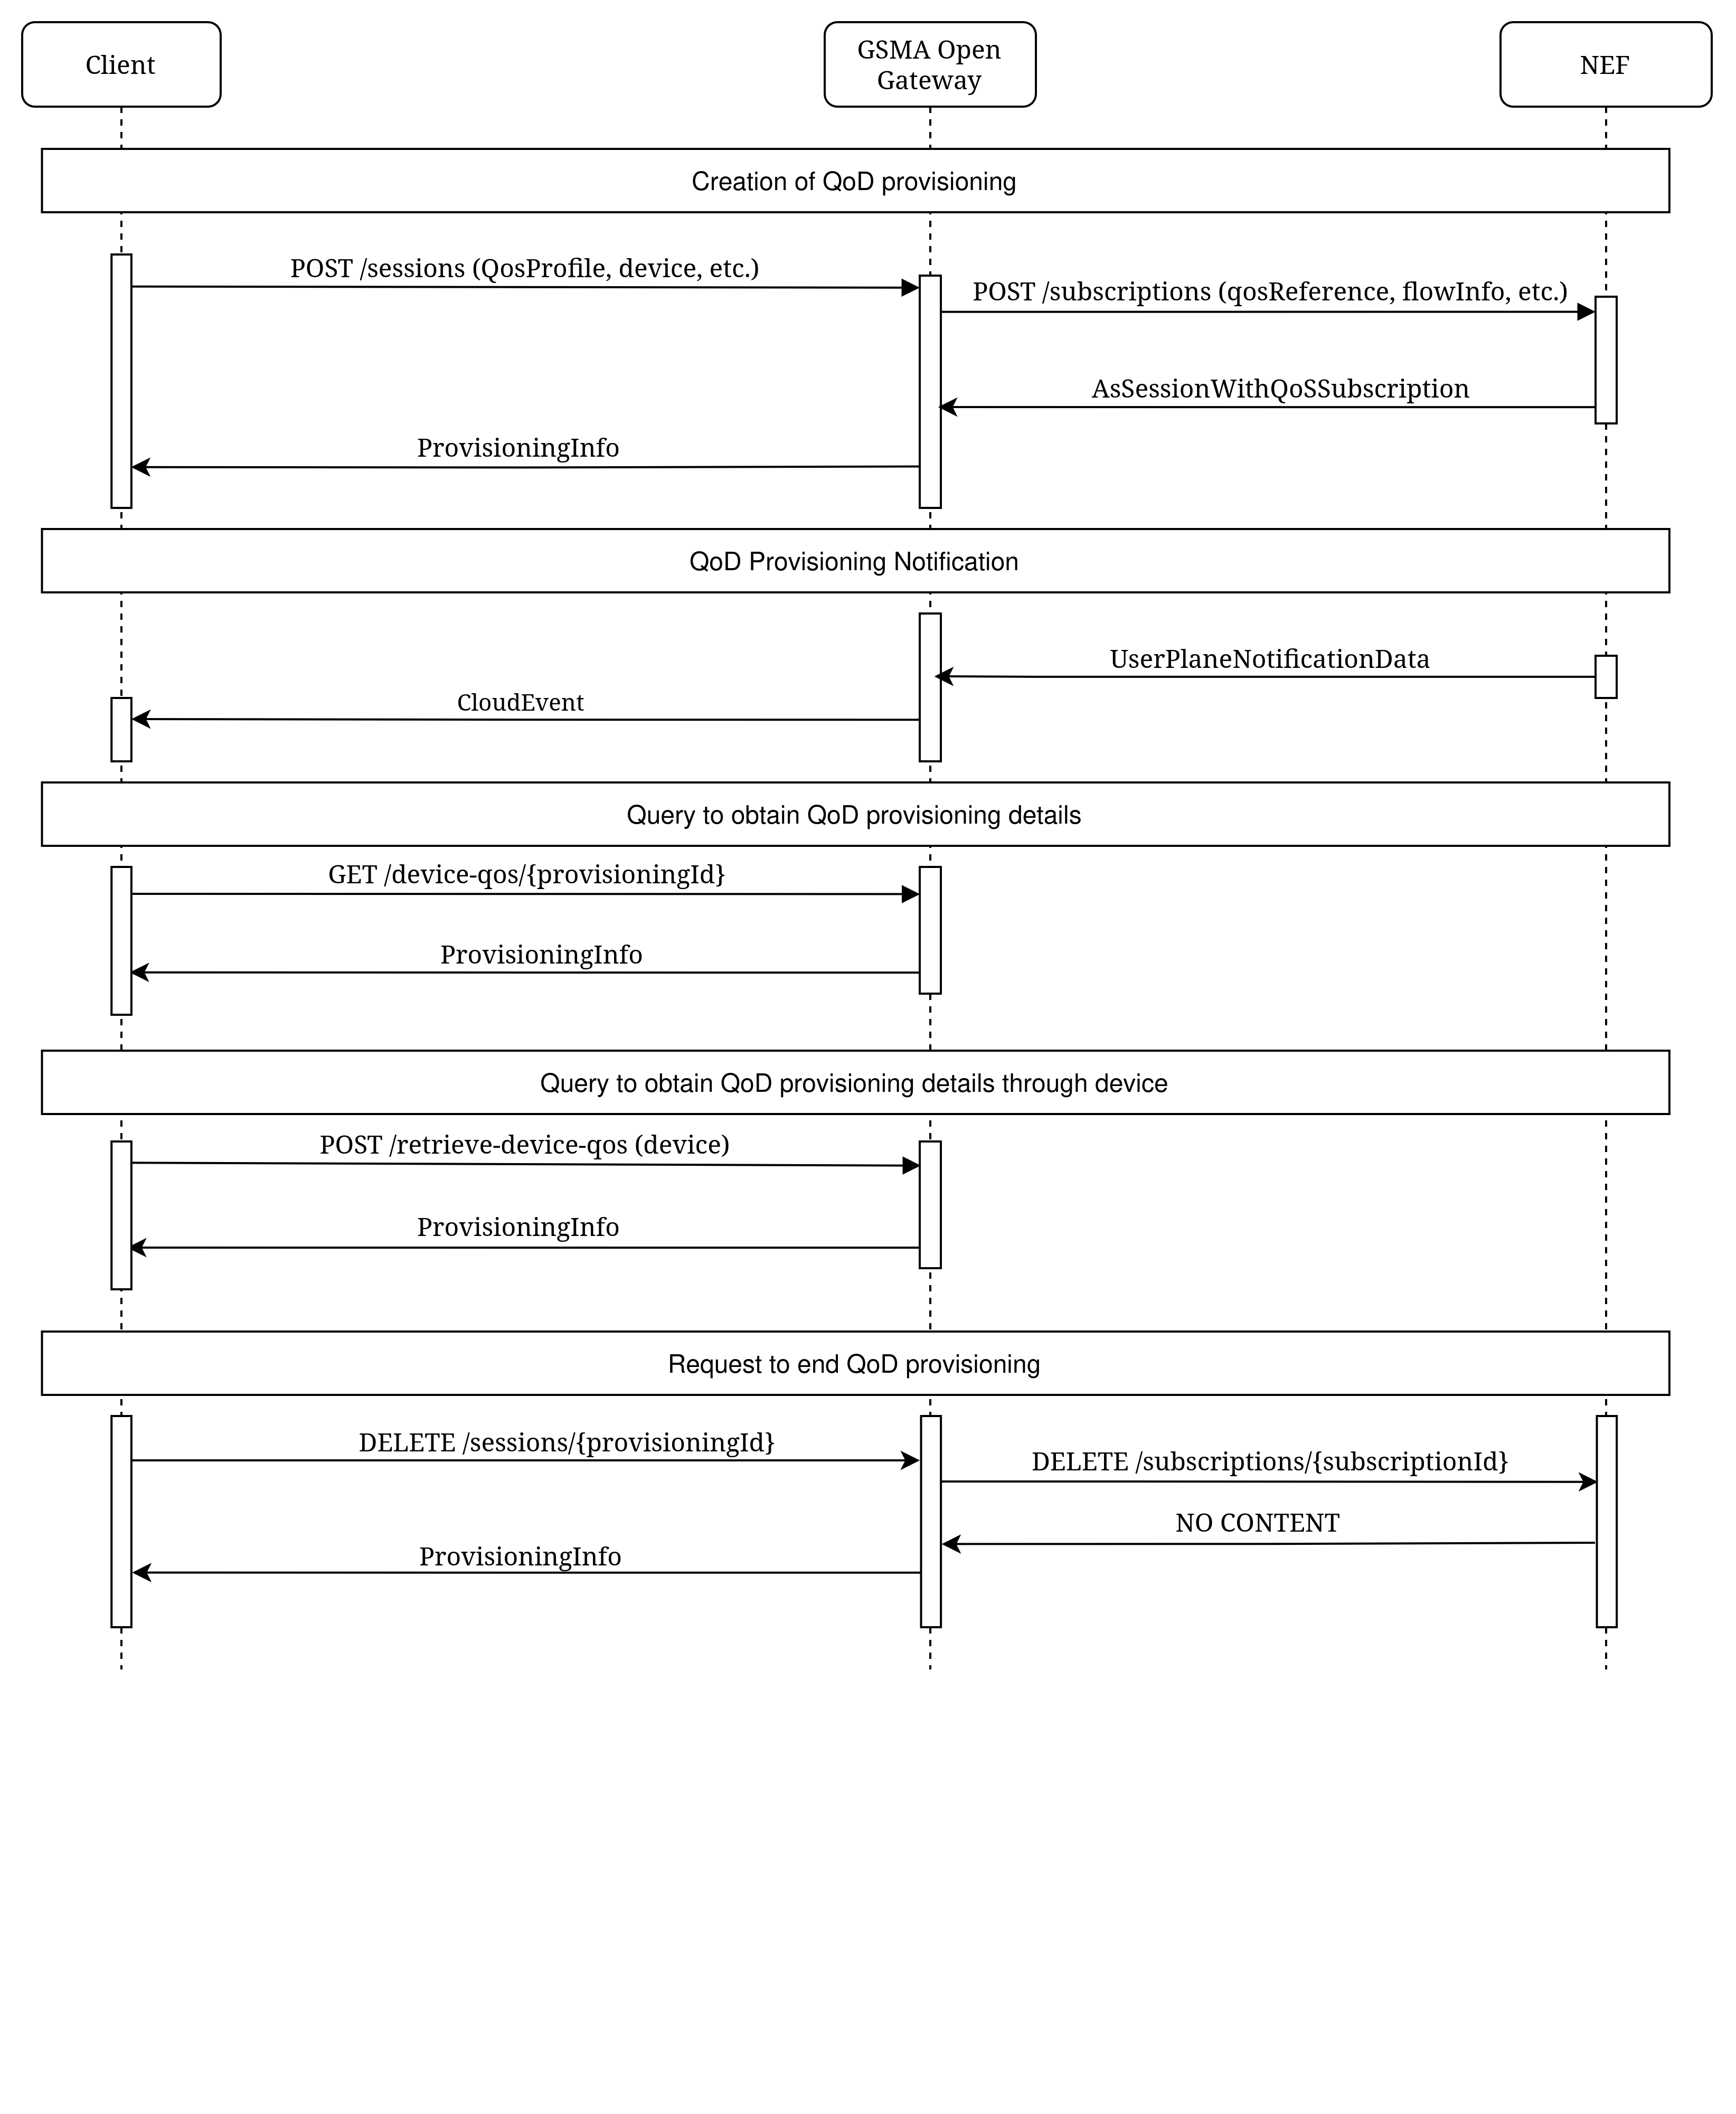
\includegraphics[width=10cm]{figs/QoD_prov_sequence_diagram.png}
	}
	\caption{Quality on Demand Provisioning Sequence Diagram}
\end{figure}

\subsection{Quality of Service Profiles}

The Quality-of-Service (QoS) Profiles API provides a collection of predefined network performance profiles, each identified by a unique name and characterized by parameters such as latency, throughput, and priority. These profiles enable application developers to define the desired network behavior for their application's data traffic, ensuring optimal and consistent performance. When used in conjunction with the Quality On Demand API, developers can request stable latency (reduced jitter) or prioritized throughput for specific data flows between client devices and application servers.

For this API, the NEF’s \emph{qosCharacteristics} interface is used to retrieve information about available QoS profiles. Depending on whether a specific QoS profile name is provided, the interface returns either the details of the requested profile or a list of all available QoS profiles and their information. The gateway processes the client’s request, making a request to the NEF interface. The NEF then responds with the corresponding QoS profile information, which the gateway then calculates the necessary parameters, and translates them into a compliant CAMARA's response, which can be used by the application to select appropriate QoS parameters for subsequent resource allocation requests.

\begin{figure}[H]
	\centerline{
		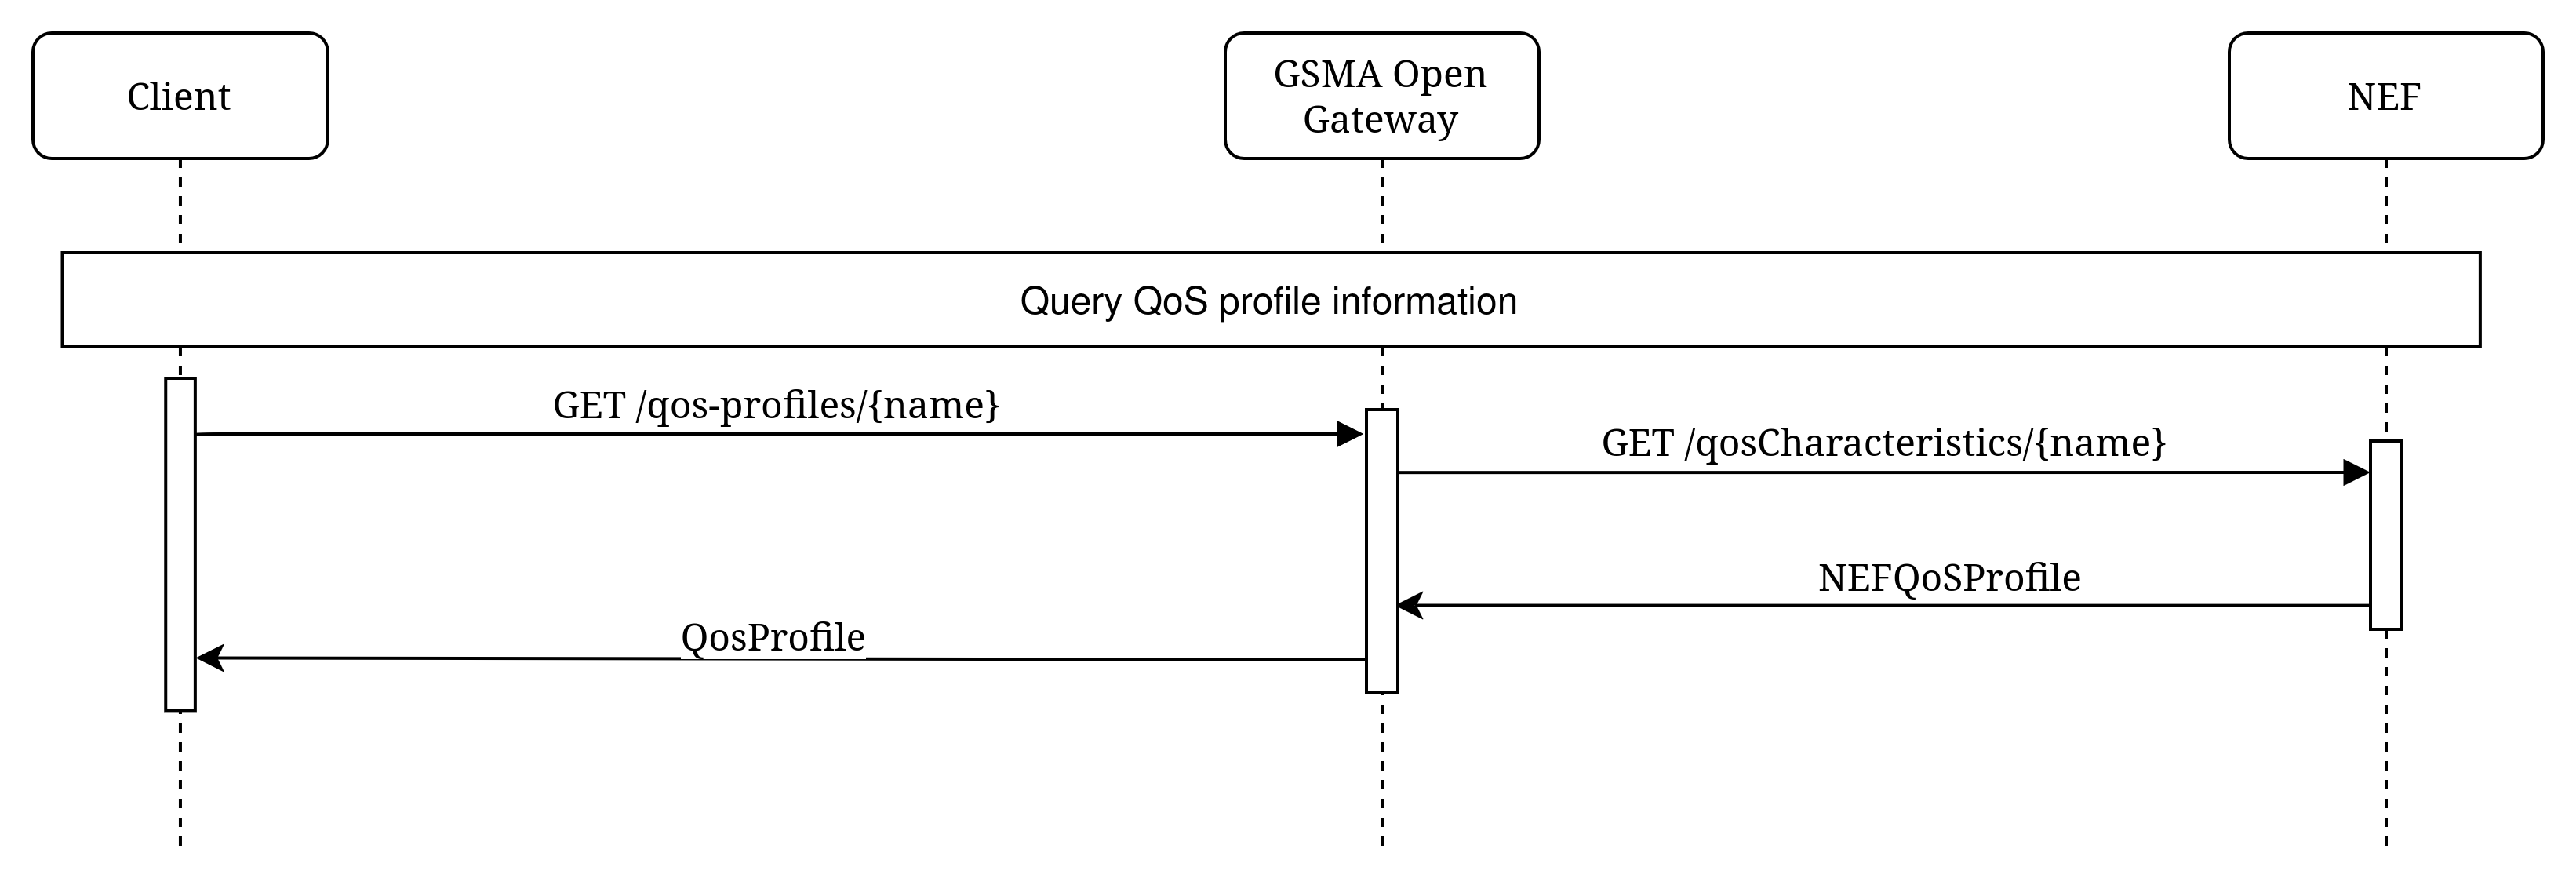
\includegraphics[width=10cm]{figs/QoS_profiles_sequence_diagram.png}
	}
	\caption{Quality of Service Profiles Sequence Diagram}
\end{figure}


\section{Device Information APIs}

We have exposed only a focused subset of the Device Information APIs on our gateway, following the same selective approach we have applied to our other API families. This decision was driven by two key factors: the current capabilities provided by IT, and our focus on addressing the core needs of our primary use cases.

Our implementation specifically supports the following APIs: Device Reachability Status, Device Reachability Status Subscription, Device Roaming Status, and Device Roaming Status Subscription. Together, these services enable us to monitor the availability of devices and track their roaming behavior in real time, while also allowing clients to subscribe to status changes proactively. This allows dependent systems to adapt to changes in device connectivity or location with minimal latency and maximum efficiency.

\subsection{Device Reachability Status}

The Device Reachability Status API enables API consumers to query the current connectivity status of a device on the mobile network. The API provides real-time information on whether a device is reachable via SMS, data (mobile internet), or both, allowing businesses to make more informed communication and service management decisions based on the device’s availability.

The implementation uses 3GPP's Monitoring Event API with the monitoring type set to \Verb{UE_REACHABILITY} with a single report and finally it also sets the reachability type to both \Verb{DATA} and then \Verb{SMS}. This means that instead of sending a notification on the next check it is sent imediatly on the response from where we extract the most recent information about both SMS and Data reachability status.

\begin{figure}[H]
	\centerline{
		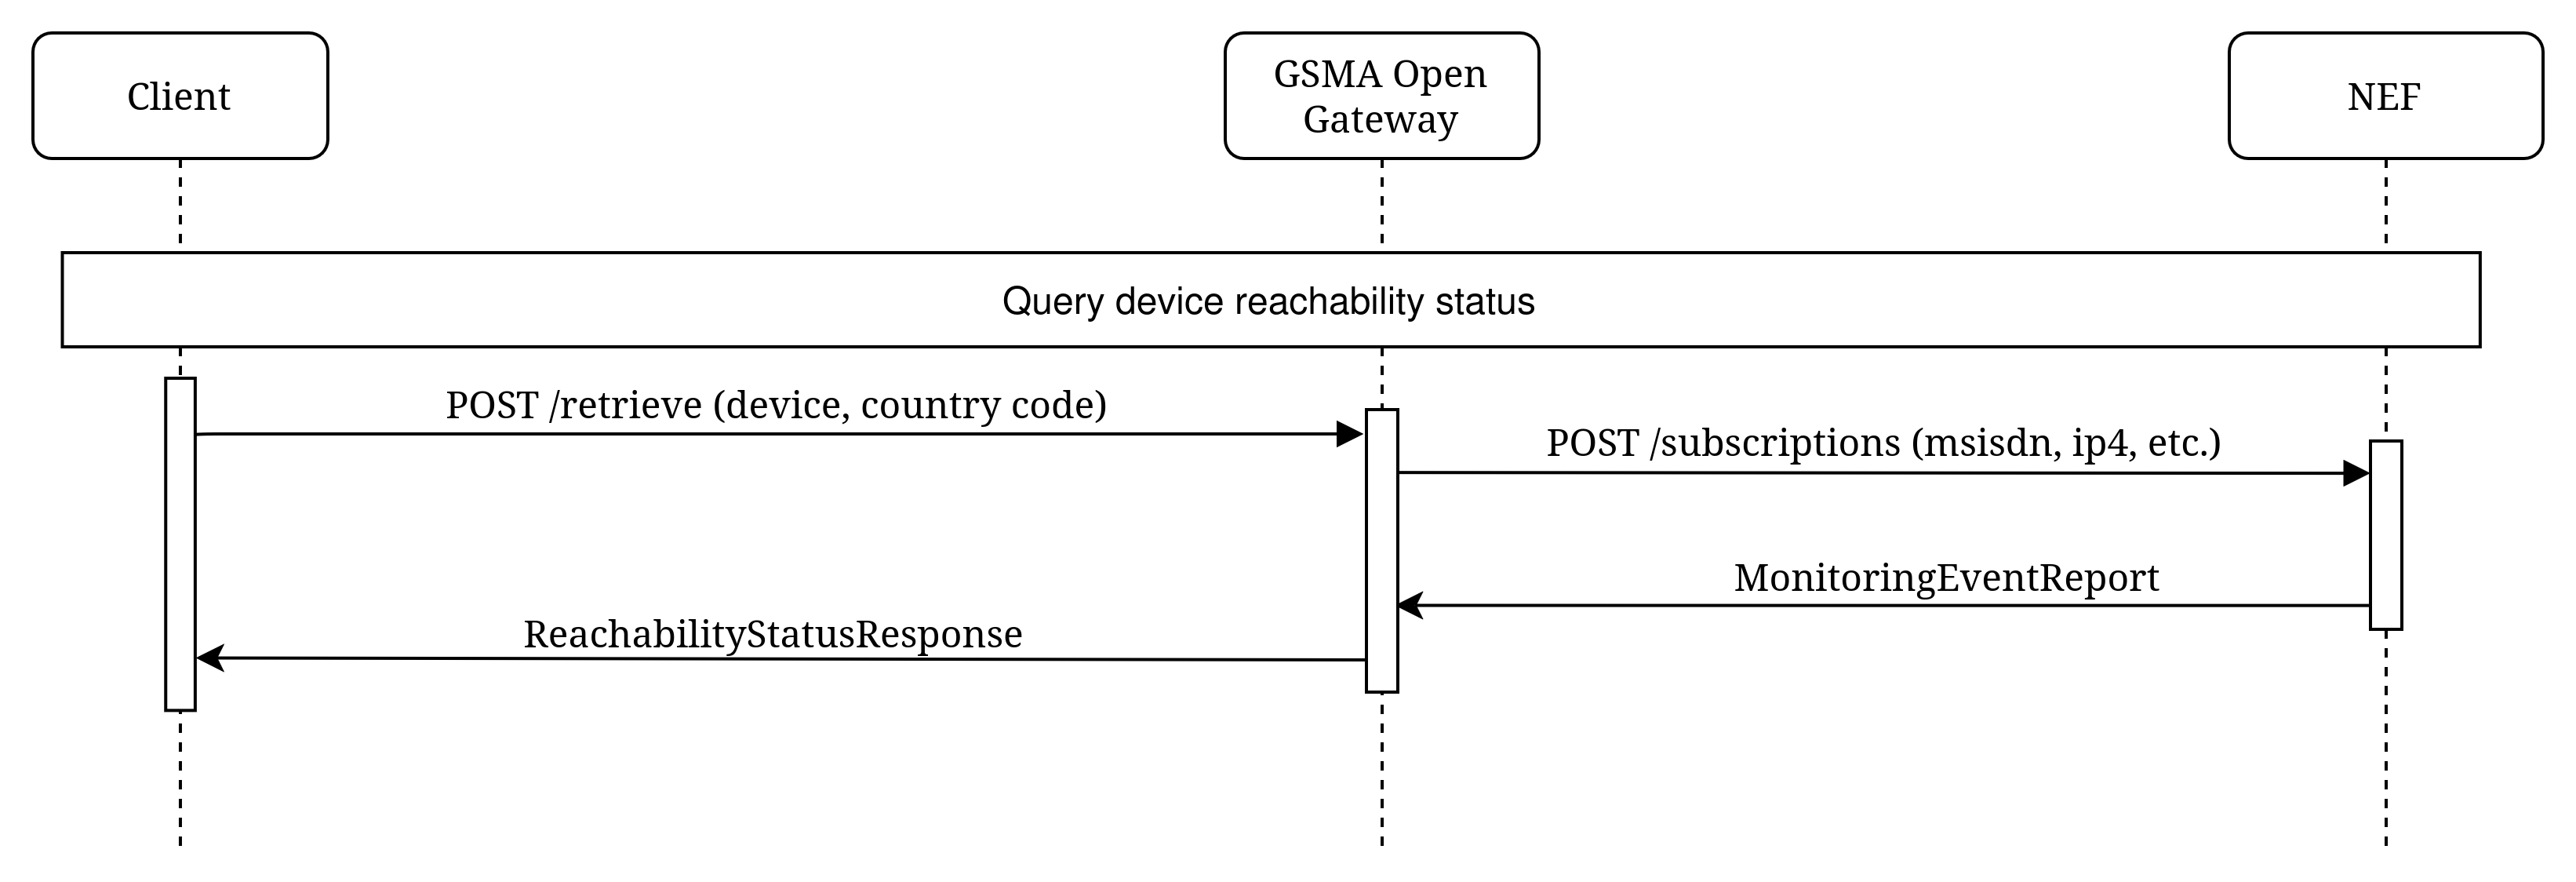
\includegraphics[width=10cm]{figs/reachability_status_sequence_diagram.png}
	}
	\caption{Device Reachability Status Sequence Diagram}
\end{figure}

\subsection{Device Reachability Status Subscription}

The Device Reachability Status Subscription API allows API consumers to subscribe to notifications about changes in a device’s connectivity status. Rather than performing repeated polling, clients can receive asynchronous updates when a device’s reachability over SMS, data, or both changes, enabling more efficient and timely service adjustments.

Our implementation leverages 3GPP's Monitoring Event API with the monitoring type set to \Verb{UE_REACHABILITY}. Unlike the one-time query used in the Device Reachability Status API, the subscription model registers an ongoing monitoring request, allowing the network to push updates whenever the reachability state changes. We configure the subscription to monitor either \Verb{DATA} or \Verb{SMS} reachability types, ensuring comprehensive coverage of the device's availability.

Furthermore, our implementation also supports retrieving the current status of all active subscriptions or querying specific subscription IDs for their details. Subscriptions can be cleanly removed via a dedicated delete operation, giving clients full control over the subscription lifecycle and resource management.

\begin{figure}[H]
	\centerline{
		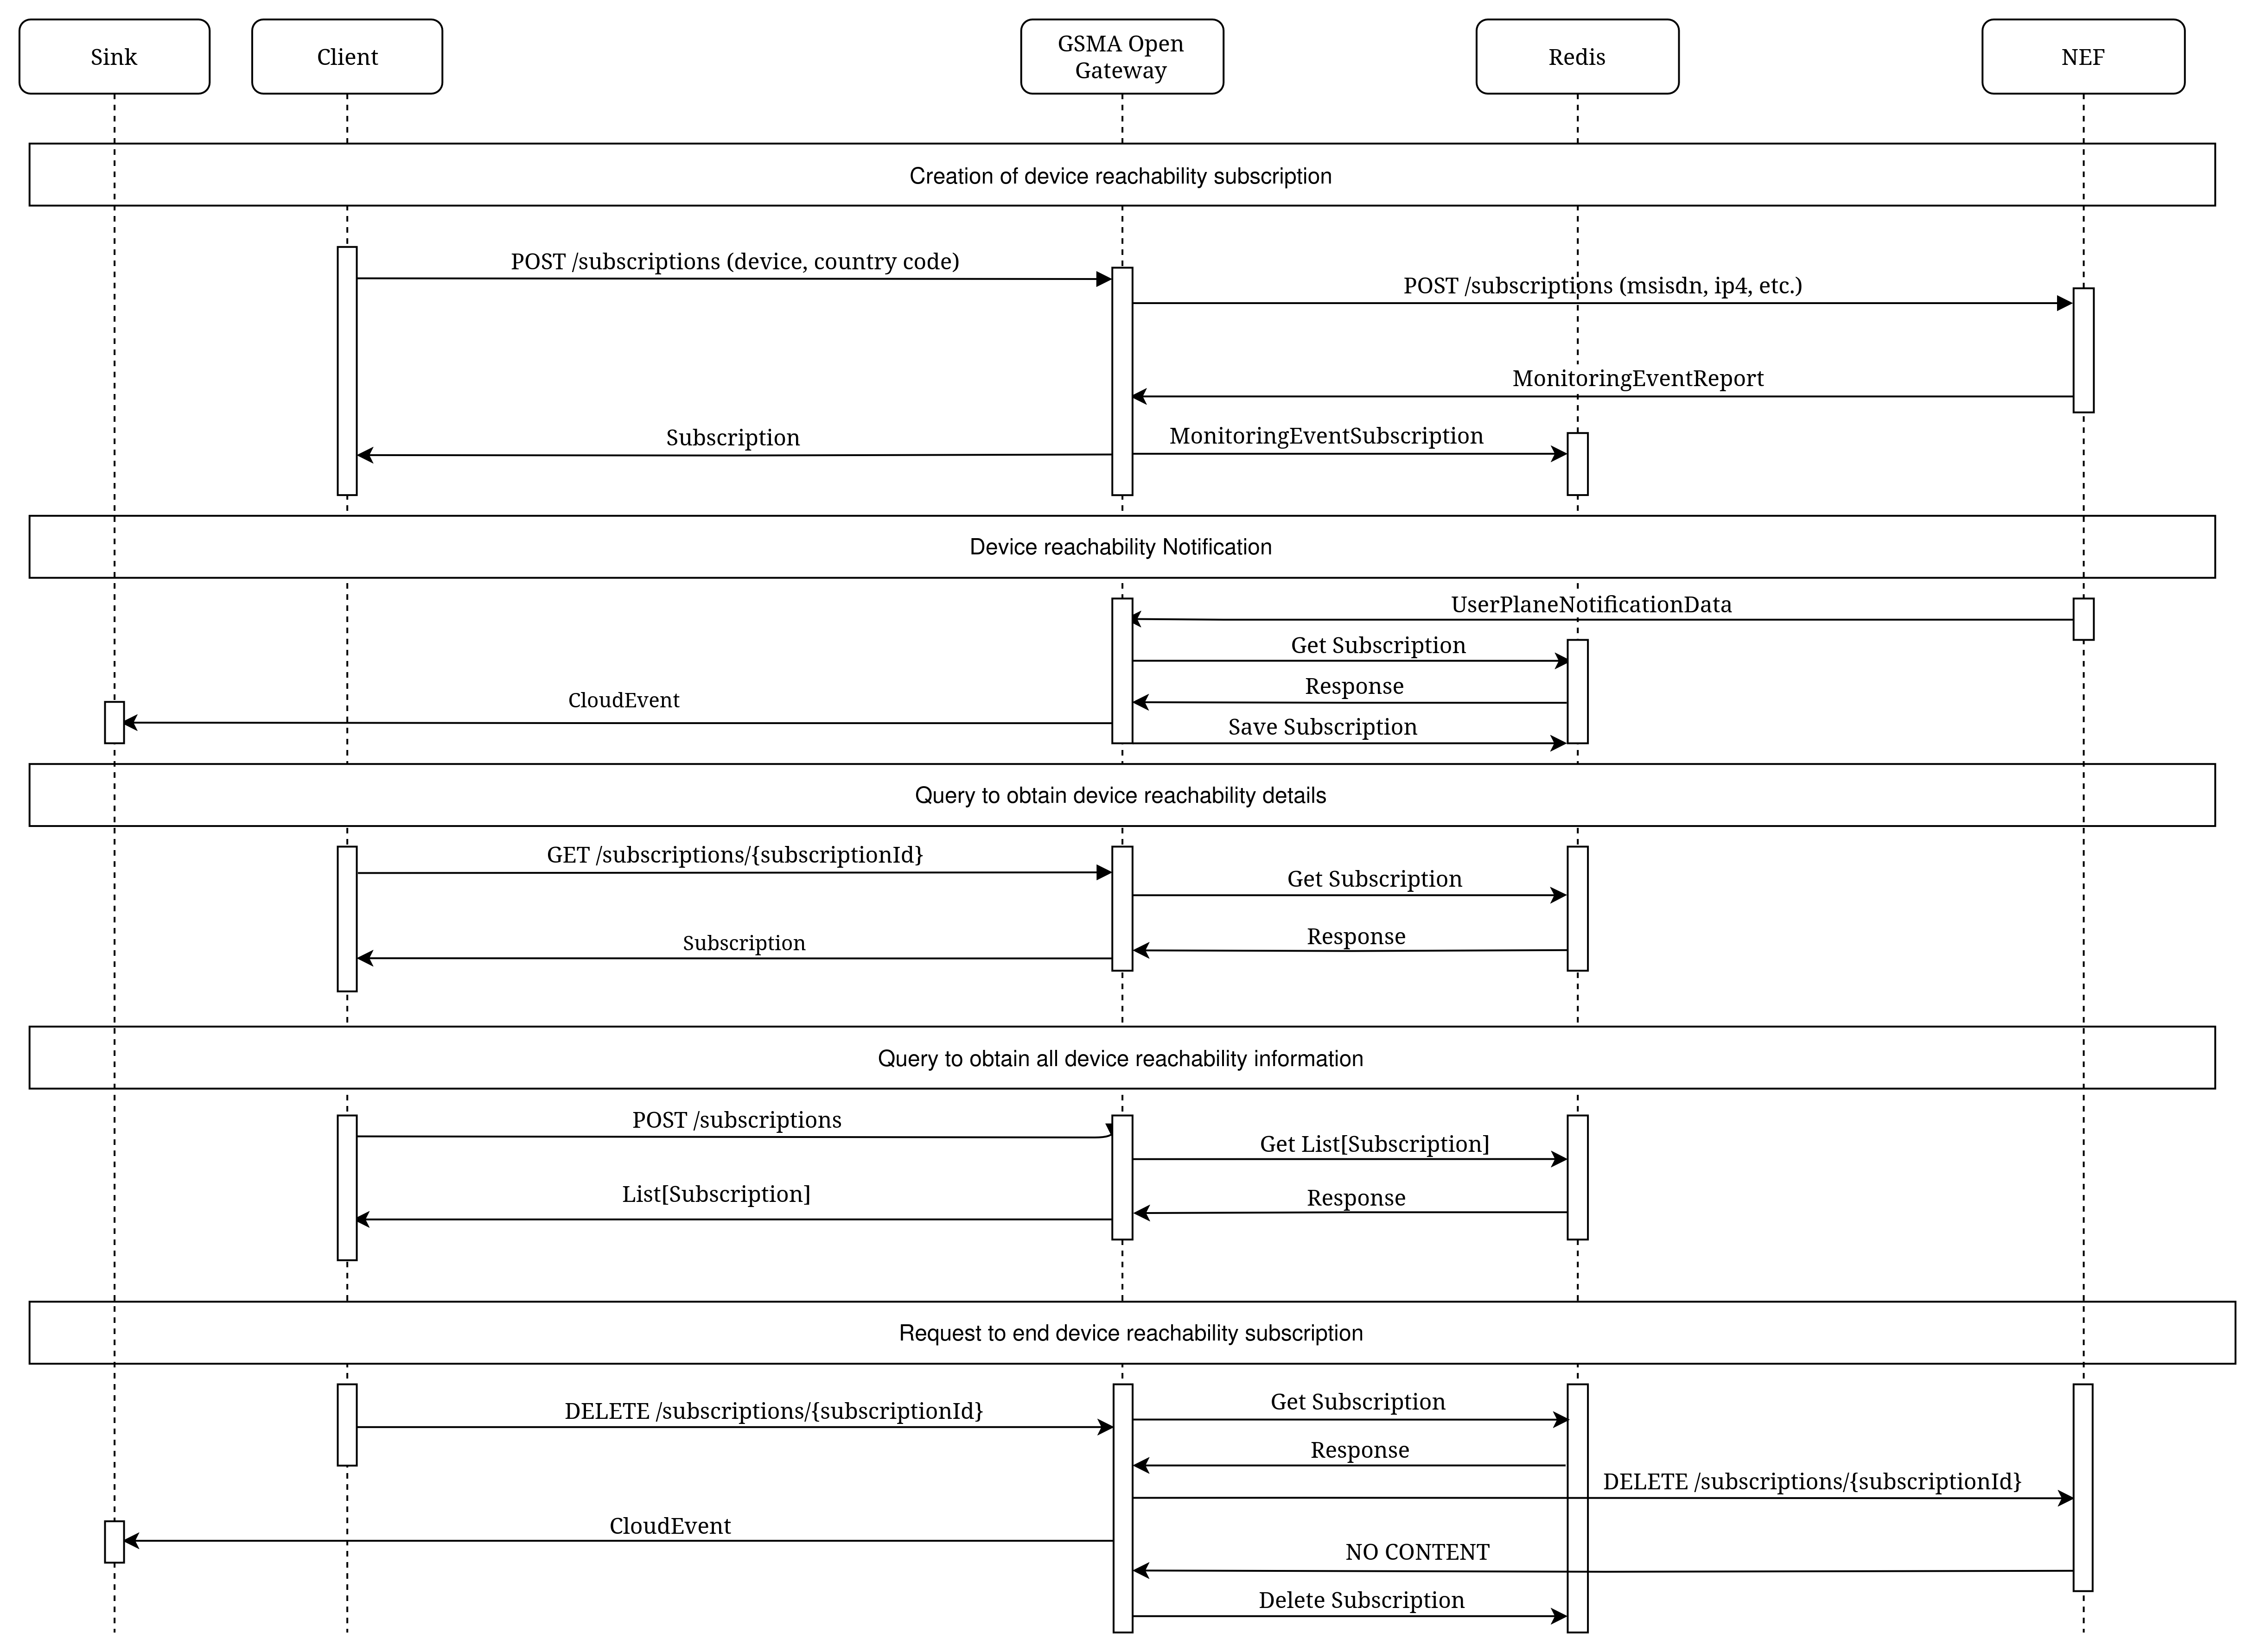
\includegraphics[width=15cm]{figs/reachability_status_sub_sequence_diagram.png}
	}
	\caption{Device Reachability Status Subscription Sequence Diagram}
\end{figure}

\subsection{Device Roaming Status}

The Device Roaming Status API enables developers to determine whether a device is roaming on a foreign mobile network and to identify the country in which it is currently located. This information supports fraud detection, regulatory compliance, and the enforcement of geo-based content restrictions.

Similar to the APIs described before, this uses 3GPP's Monitoring Event API, however the monitoring type is set to \Verb{ROAMING_STATUS} and with a single report. This means, like the Device Reachability Status API, the information is sent imediatly on the response from where we get the most recent information about the device's roaming status

\begin{figure}[H]
	\centerline{
		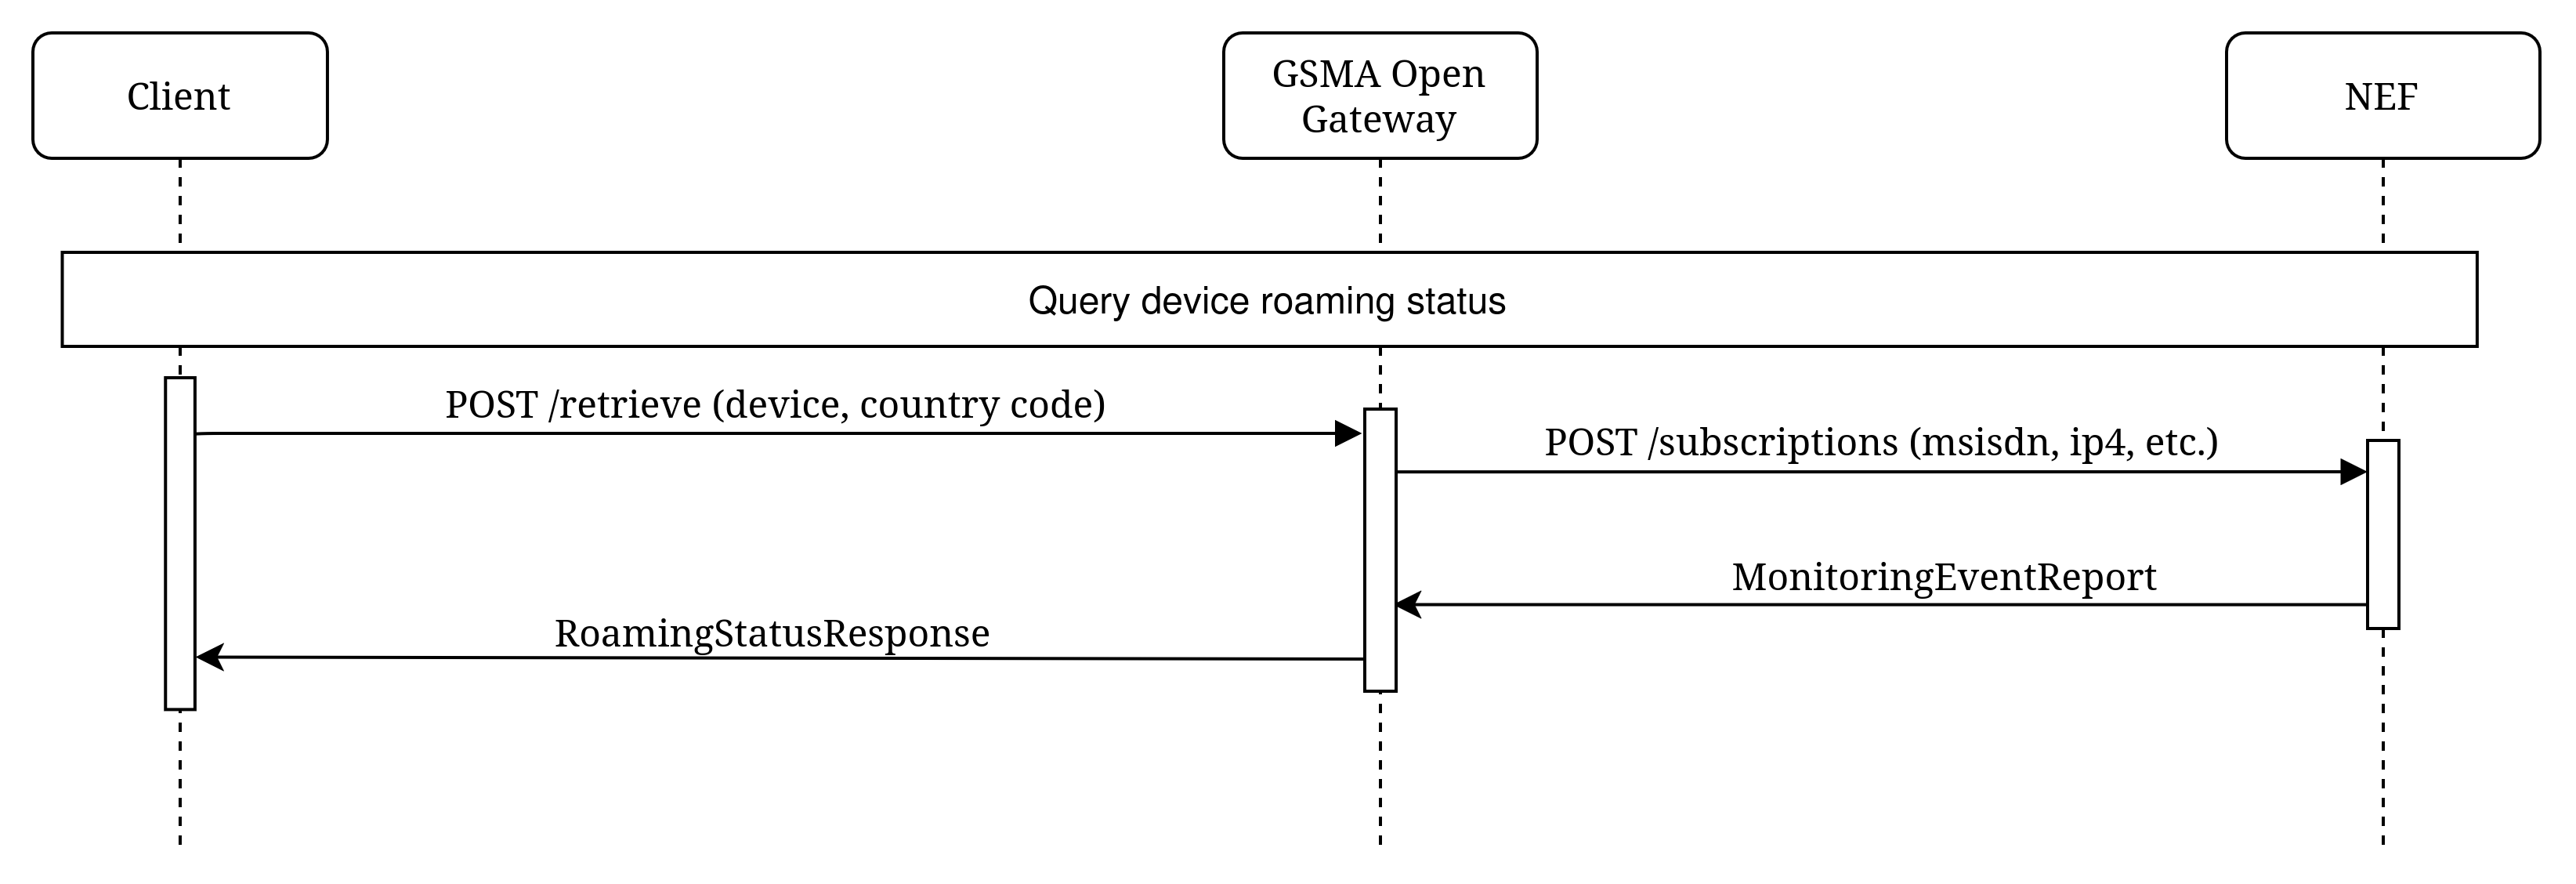
\includegraphics[width=10cm]{figs/roaming_sequence_diagram.png}
	}
	\caption{Device Roaming Status Sequence Diagram}
\end{figure}

\subsection{Device Roaming Status Subscription}

The Device Roaming Status Subscription API allows API consumers to receive asynchronous notifications whenever a device’s roaming status changes. This eliminates the need for repeated polling, enabling real-time awareness of roaming events that can be critical for fraud detection, regulatory enforcement, and geo-based service adjustments.

Our implementation is based on 3GPP's Monitoring Event API with the monitoring type, once more, set to \Verb{ROAMING_STATUS}. Unlike the one-time query used in the Device Roaming Status API, the subscription model establishes an ongoing monitoring request, allowing the network to proactively notify clients whenever the device's roaming state changes. Each update includes the roaming status, providing accurate and timely context for decision making.

In addition to subscribing, API consumers can retrieve a list of all active subscriptions or query specific subscription IDs to inspect their current configuration. Subscriptions can also be deleted as needed, allowing clients to efficiently manage resources and control subscription lifecycles.

\begin{figure}[H]
	\centerline{
		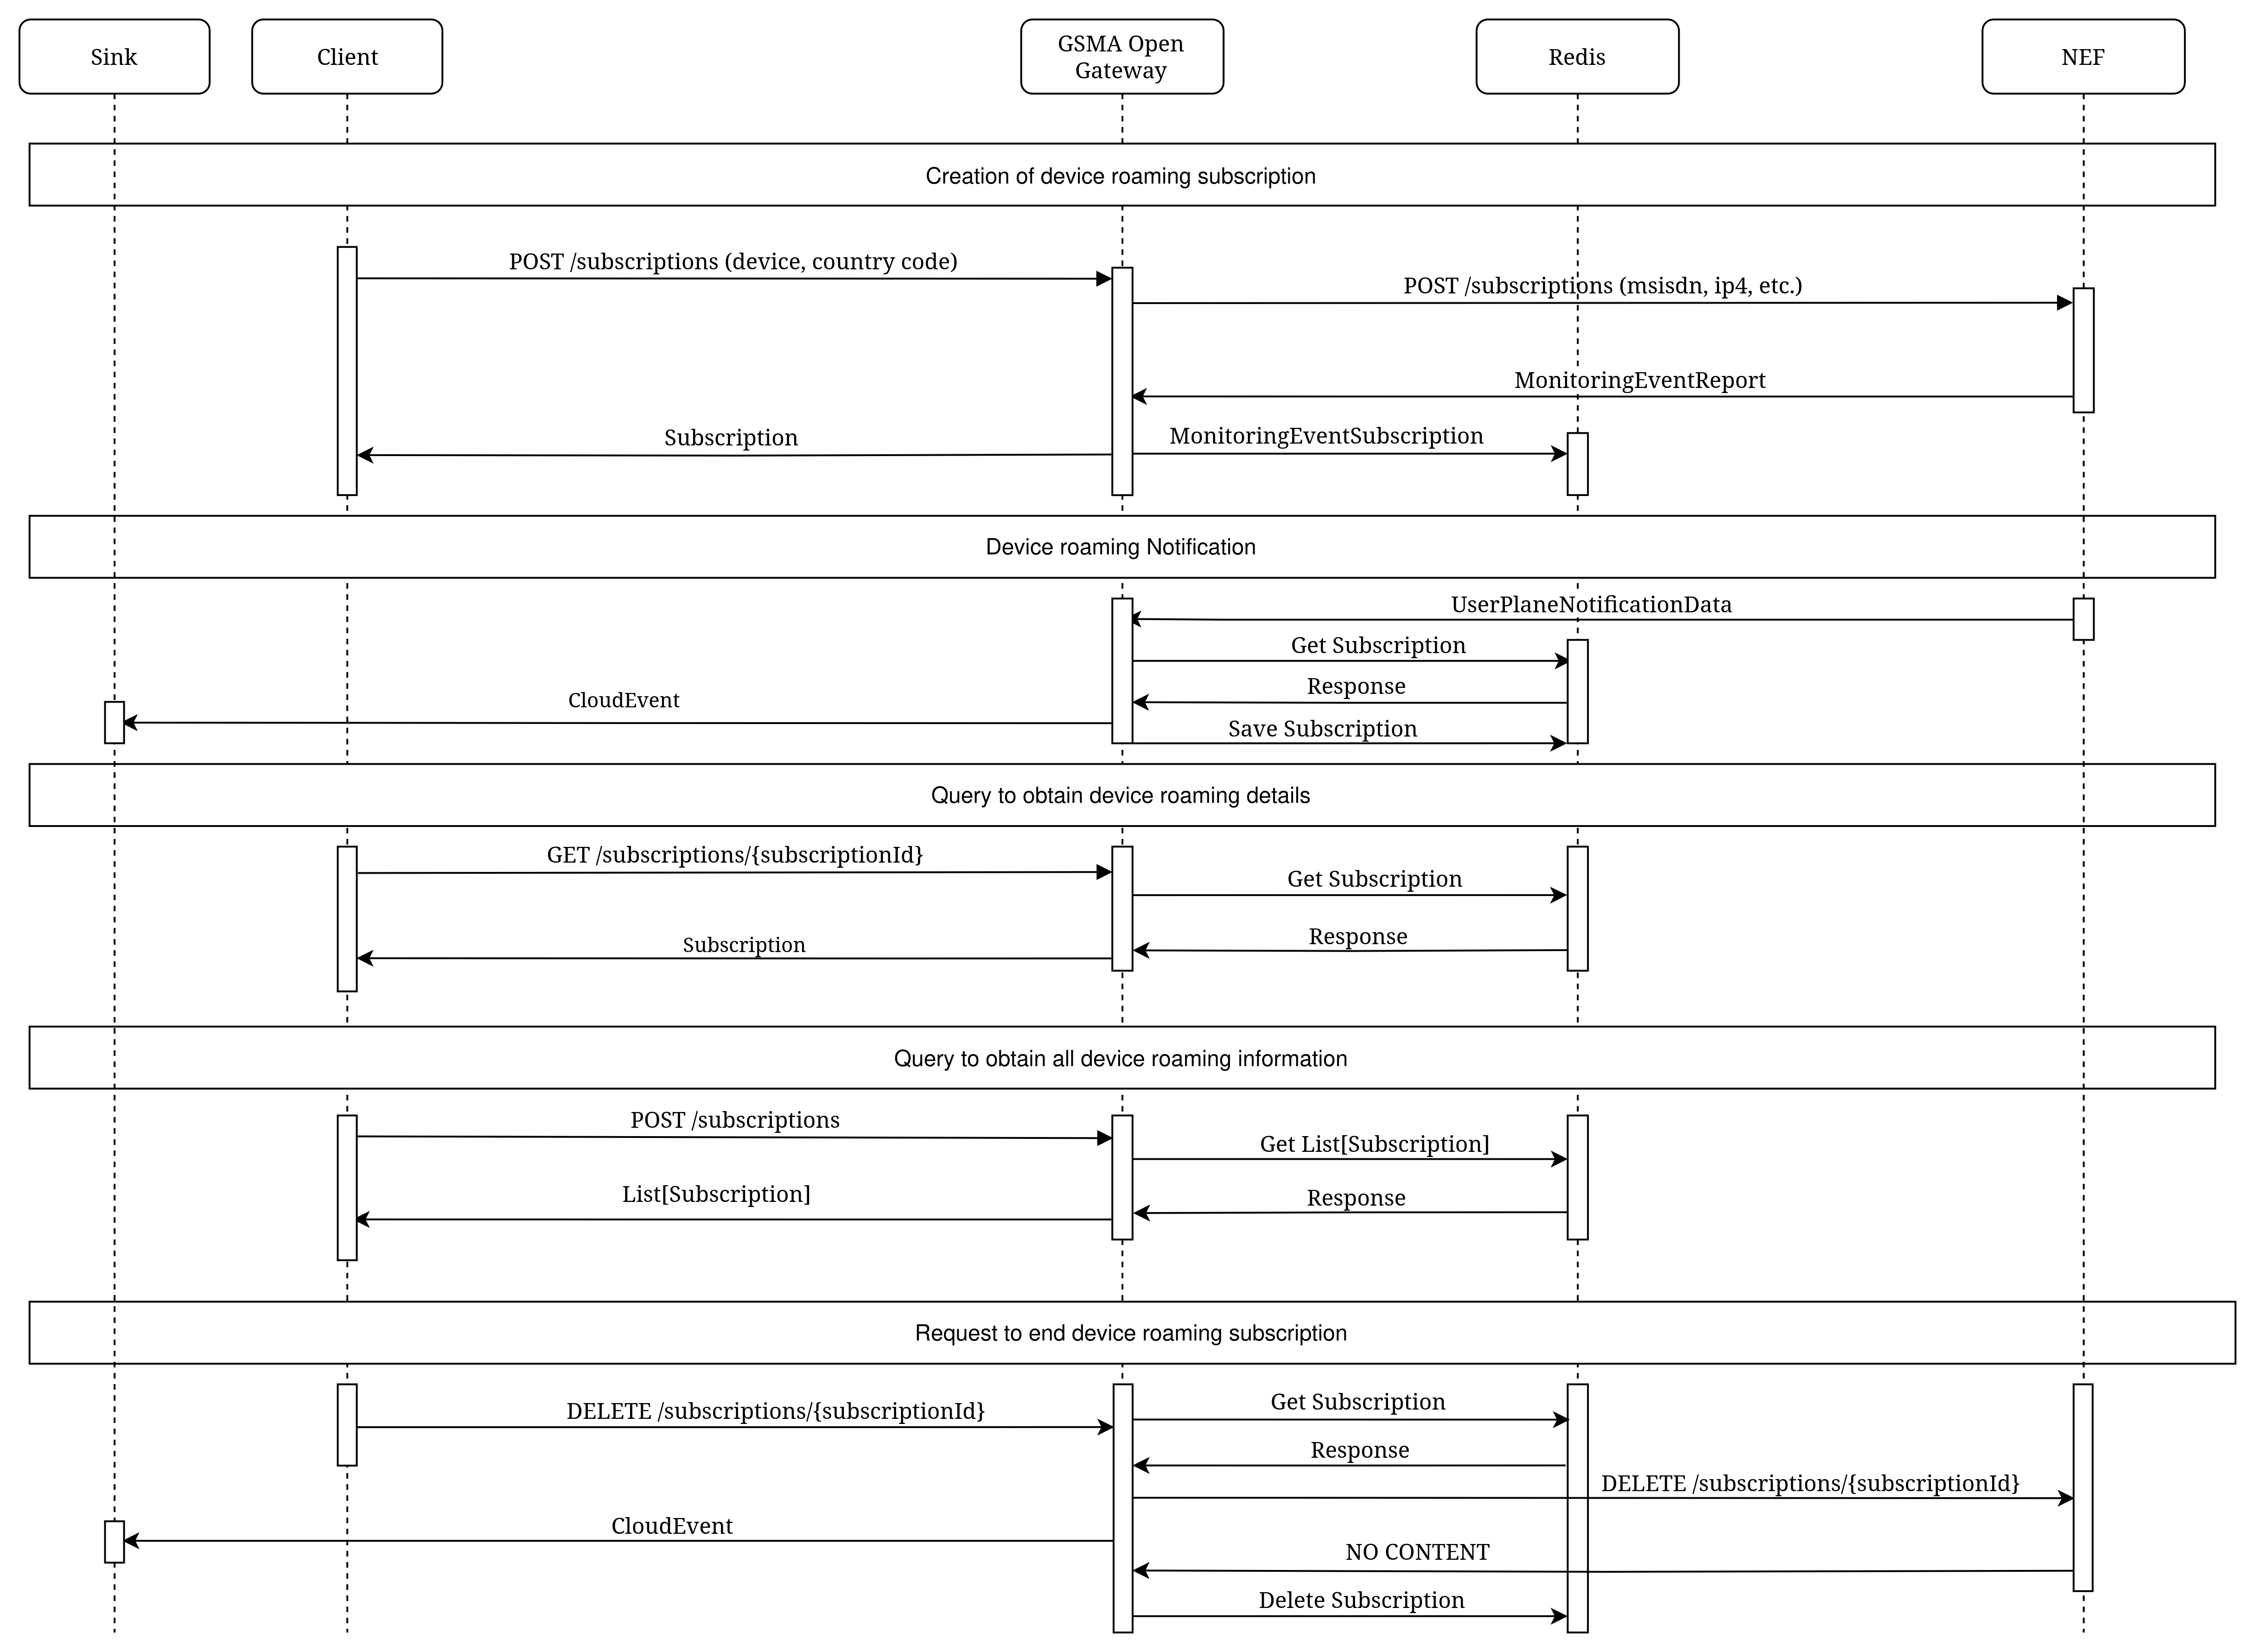
\includegraphics[width=15cm]{figs/roaming_sub_sequence_diagram.png}
	}
	\caption{Device Roaming Status Subscription Sequence Diagram}
\end{figure}

\section{Authentication and Fraud Prevention}

This group of APIs specializes in authenticating devices and preventing fraud.
Here we identified one API that was achievable with the available
infrastructure, (even though we had to complete it), and that was the One Time
Password SMS API.

\subsection{One Time Password SMS}

This API consists of two main steps, sending a One Time Password (OTP) via SMS
and verifying wether the result was correct or not, therefore we have two
endpoints, one for each action.

When calling the send OTP endpoint a couple things happen. First an
authentication ID is generated in order to be able to verify the code, since it
is required to use this authentication ID in the verification step to be able
to associate the code stored with the code received by the device. Then the
code itself is generated. At this point we store the code and replace the
placeholder in the message to be sent with the real code. The code is not
stored in plain text for security reasons, instead a hash of the code is
stored. The final step is to send the actual SMS with the message and the code,
this is done by calling an SMSC's endpoint.

At this stage in the process the code has been sent to the desired device and
all information has been stored. In order to complete the verification the
verification endpoint must be called with the code received on the device. The
endpoint must also be called with the authentication ID in order to be able to
associate the received code with an authentication attempt. From here two
possibilities arise, either the code is correct and the authentication succeeds
or the code is incorrect and after some number of failed attempts the code gets
removed and a new authentication cycle needs to start. The verification step
requires the code that is being verified to be hashed, and for security reasons
the comparison is done in constant time to prevent timing attacks.


\section{CAMARA as a Service}


\chapter{Auxiliary Development}
\section{The Kamailio Project}
\section{The NEFEmulator Project}
\section{IT Infrastructure Integration}



\chapter{Roadblocks}


\chapter{Results}


\chapter{Future Work}


\chapter{Conclusion}



\printbibliography[heading=bibintoc]

\end{document}
